\subsection{Preprocessing}
\subsubsection{Kuwahara filter}
\begin{figure}[htb!]
\centering
\begin{subfigure}{.24\textwidth}

\includegraphics[width=\textwidth]{images/miku_d.png}
\caption{Before filtering.}
\end{subfigure}
\begin{subfigure}{.24\textwidth}

\includegraphics[width=\textwidth]{images/miku_d_filtered_smallh.png}
\caption{Small window.}
\end{subfigure}
\begin{subfigure}{.24\textwidth}
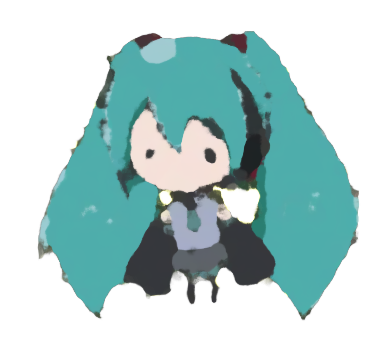
\includegraphics[width=\textwidth]{images/miku_d_filtered.png}
\caption{"good" window.}
\end{subfigure}
\begin{subfigure}{.24\textwidth}
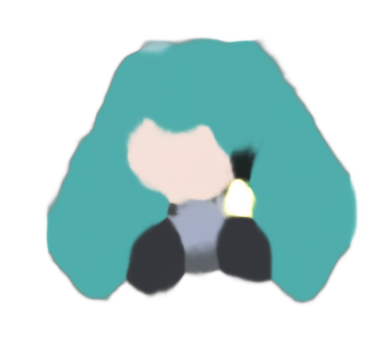
\includegraphics[width=\textwidth]{images/miku_d_filtered_largeh.png}
\caption{Large window.}
\end{subfigure}
\caption{Results of Kuwahara filtering with varying window size. The small window causes outlines to be accentuated, and the large window removed the tie, ribbon and legs.}
\label{fig:kuwaharaExample}
\end{figure}

One of the early issues encountered when attempting to segment animation character images was the presence of black outlines, which usually get segmented into many large components, but do not contain any information relevant to identification. We identified the Kuwahara filter \cite{kuwahara1976processing} as a way to not only remove the black outlines, but also remove other unnecessary details and make area of color more homogeneous and amenable to segmentation.

\paragraph{The method} Consider a grayscale image $I$ (we'll see later how it generalizes to color images). For each point $(x,y)$ on $I$, we consider a square window of size $2h + 1$ centered on it. We then consider $4$ overlapping square regions in this window as shown in \autoref{fig:kuwaharaQuadrants}. For each such region $Q_i$ for $i \in \{1, ..., 4\}$ we compute the arithmetic mean $m_i(x,y)$ and standard deviation $\sigma_i(x,y)$ of pixel values inside $Q_i$. The pixel value at $(x,y)$ in filtered image $J$ is then defined as the arithmetic mean $m_i(x,y)$ corresponding to the smallest standard deviation $\sigma_i(x,y) = \min_{j \in \{1, ..., 4\}}\sigma_j(x,y)$. When dealing with borders of the image, we simply do not consider the missing pixels while computing the means and variances.

\begin{figure}[htb!]
\centering
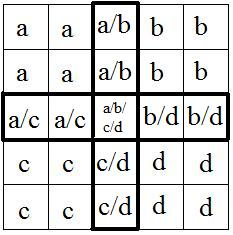
\includegraphics[width=0.3\textwidth]{images/kuwahara_quadrants.jpg}
\caption{Window used by the Kuwahara filter with half-size $h = 2$ and square regions $a$, $b$, $c$ and $d$.}
\label{fig:kuwaharaQuadrants}
\end{figure}

Generalizing to color images, we still consider the arithmetic means of pixel colors, but this time we consider the brightness of the pixels (e.g. the V in HSV color space) for standard deviation.

\paragraph{Theoretical justification} The algorithm was originally designed to improve segmentation in medical image processing. For the case of removing outlines, if one considers a window size "large enough" that outlines never fills most of it, then it will introduce a large standard deviation in the square region it is contained in - meaning it will be removed in the filtered image. It should be noted that if the window is not large enough, then outlines can actually be thickened by the Kuwahara filter, and if it is too large then relevant information may be lost (\autoref{fig:kuwaharaExample}). We found however that it is easy do empirically determine a window size in practice.

\paragraph{Implementation} A naive implementation of the filter recomputes all means and variances for each pixel, runs in $O(nh^2)$ time where $n$ is the number of pixels in the image, and $h$ is the window half size.

\subsubsection{Color space selection}

As the goal is to obtain a segmentation as close to human perception as possible, the $L^*a^*b^*$ color space has been found to be most suitable. The $HSV$ or $HSL$ color spaces are also useful to extract hue information, (the $H$ in either color space) which we use for histogram equalization (\autoref{sec:histEq}) and as post-processing to segmentation (\autoref{sec:hueMerging}).

Although using $L^*a^*b^*$ color space gives good segmentations, it may not be ideal for classification as $2$ different characters may share predominantly the same color palette. A possible extension of this would be to use training data to determine an abstract and possibly non-linear color space where members of the same class are close and members of different classes are far away, using - for instance - a (semi) supervised embedding method similar to the one used in \cite{urahama2007semi}.

\subsubsection{Color histogram equalization by hue}
\label{sec:histEq}

Some characters are represented predominantly by a few colors, which makes segmentation more difficult. Equalizing the histogram by hue allows segmentation to distinguish between more closely related colors, and therefore distinguish some colors which would be otherwise close in color space. The drawback beinng that irrelevant differences in color space are also accentuated, so histogram equalization was eventually removed from preprocessing as it had an overall negative impact on segmentation performance.